\documentclass[a4paper,10pt]{article}
\usepackage[utf8]{inputenc}
\usepackage[T1]{fontenc}
\usepackage[french]{babel}
\usepackage[final]{pdfpages}
\usepackage{verbatim}
\usepackage{hyperref}
\usepackage{color}

\usepackage[top=1.5cm, bottom=1.5cm, left=1.45cm, right=1.45cm]{geometry}

\newcommand{\HRule}{\rule{\linewidth}{0.5mm}}

\begin{document}

\begin{titlepage}

  \begin{center}

% Upper part of the page

    \textsc{\Large Universite Catholique de Louvain}\\[1cm]

    \textsc{\LARGE{Databases}}\\[1cm]


% Title
    \HRule \\[0.35cm]
    {\huge \bfseries Mission 4: Database Programming \\ The Automated Cafe}\\
    \HRule \\[0.35cm]
        \end{center}
      \begin{figure}[h!]
      \begin{center}
       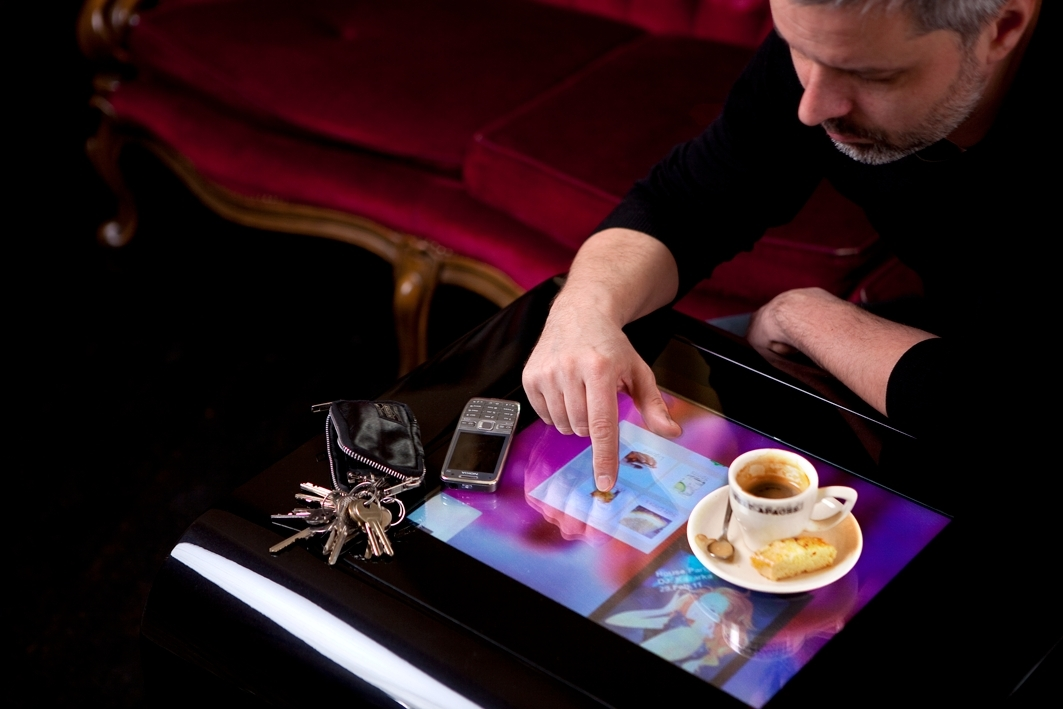
\includegraphics[scale=0.6]{restaurant.jpg}
      \end{center}
      \end{figure}

    \begin{center}
    \HRule \\[0.2cm]
  \end{center}

    \begin{minipage}{0.48\textwidth}
      \begin{flushleft} \large
        \textit{Auteurs:}\\
        Jonathan \textsc{Powell} (61331200)\\ \vspace{0.3cm}
        Jérôme \textsc{Lemaire} (69601000)\\ \vspace{0.3cm}

        \textit{Cours:} \\
        LINGI2172 \\ \vspace{0.3cm}
         \textit{Groupe:} \\
         Query builder 20
        

      \end{flushleft}
    \end{minipage}
    \begin{minipage}{0.48\textwidth}
      \begin{flushright} \large
        
       
        \textit{Titulaire:} \\
        Bernard \textsc{Lambeau}\\ \vspace{0.3cm}
        \textit{Assistants:} \\
        Antoine \textsc{Cailliau}\\
        Quentin \textsc{De Coninck}\\
        
      \end{flushright}
    \end{minipage}

    \vfill
% Bottom of the page

    \begin{minipage}{0.3\textwidth}
      \begin{flushleft}
        
\includegraphics[height=2cm]{logo_UCL.jpg}
      \end{flushleft}
    \end{minipage}
    \begin{minipage}{0.3\textwidth}
      \begin{center}
        {\large INFO21}\\
        {\large \today}
      \end{center}
    \end{minipage}
    \begin{minipage}{0.3\textwidth}
      \begin{flushright}
        
\includegraphics[height=2cm]{logo_EPL.jpg}
      \end{flushright}
    \end{minipage}
\end{titlepage}

\section*{Introduction}

As part of the course LINGI2172, we realized different approach to organize the database of the Automated Café application. In this report you will find a small summarize of the work done for this project. In the main directory of the project there is a \texttt{Readme.md} file, don't forget to have a look to know how to run the different parts of the project. There is also different scenarios files that can be ran to test our models. The project was divided in three different steps and we will discuss in this report the realization done for each of these parts.

\section*{Structure of database}

The structure of the database stays the same for each step. The Figure 1 below shows the different relvars. \\

\begin{figure}[h!]
      \begin{center}
       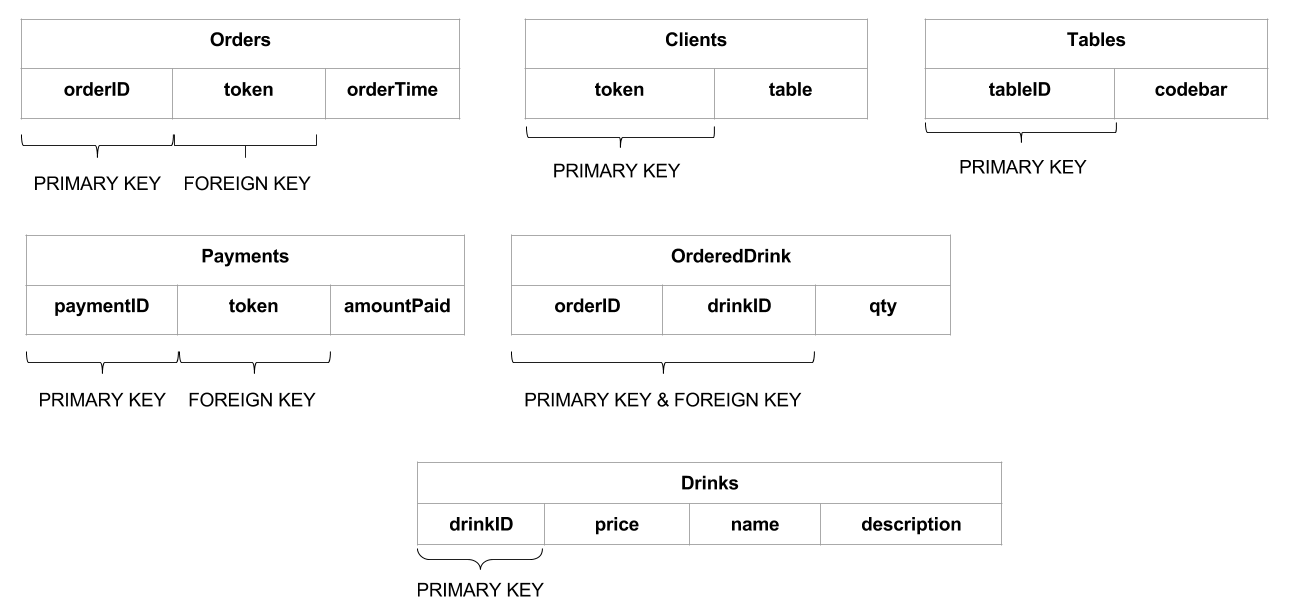
\includegraphics[scale=0.4]{relations.png}
       \label{rel}
       \caption{Relations : Structure of the database}
      \end{center}
\end{figure}

In the relation \texttt{Clients} each token must unique, this is why we use it as the primary key. Each single primary key are incremented automatically as well for the step 1 and step 2 that for the step 3. The relvar \texttt{Clients}, \texttt{Orders}, \texttt{Payments} and \texttt{OrderedDrink}, as shown on the Figure 1, also have foreign keys. We also added constraint on the column \texttt{qty}, \texttt{price} and \texttt{amountPaid} since they represent quantity and money they must be equals or greater than 0.

\section*{Step 1}
The files in this step are in the directory \texttt{database}. The most interesting file to analyze is the file \texttt{procedures.sql}. The language used is \texttt{PL/pgSQL}. It contains the definition of type, storage procedure, view and trigger. description of the four major procedural functions : 
\begin{description}
\item [AcquireTable] allows to add a customer in the \texttt{Clients} table if the table is free. To check if the table is free to insert before a customer in the table \texttt{Clients}, we implemented a trigger on \texttt{Clients}. If the table is not free, we display an error message. A table is free if the number of the customer sitting in this table is equals to the number of the payment in this table.
\item[OrderDrinks] simulates the drinks order. A drink order is represented by the type \texttt{orderList}. \texttt{OrderList} represent a tuple (drinkid, quantity of drink). The \texttt{OrderDrinks} procedure insert the order in the table \texttt{Orders} and \texttt{OrderedDrink}.
\item[IssueTicket] is call when the customer will ask for the bill. We implemented the view \texttt{bill} which contains all the drinks ordered but not yet paid for all the table occupied by a client. The function \texttt{IssueTicket} returns the total amount of the orders and a list of \texttt{ordernameList} for the customer. The \texttt{ordernameList} type represent the tuple (drinkname, quantity).
\item[PayTable] is call when the customer will pay and free his table. First, we check if the token is valid and the table is occupied with the function \texttt{is\_valid\_token}.  Note that this function is also use in the \texttt{OrderDrinks} and \texttt{IssueTicket} procedures. Finally before updating the database, we check that the payment is greater than the amount due.

\end{description}

\section*{Step 2}
The files in this step is in the directory \texttt{call-level-api}.
We implement the call-level \textsc{api} with the library \texttt{Psycopg2} in \texttt{Python}. It calls the procedures implemented in the step 1. 
\section*{Step 3}

We use Django as higher-level approach to database connectivity, more precisely we are going through a framework named Django-Query-Builder \footnote{Django-Query-Builder version 0.10.0 : \url{https://pypi.python.org/pypi/django-query-builder}}. Django-Query-Biulder is a Python library that allows us to construct and execute SQL instruction in query builder mode. This part of the project are in the directory \texttt{query-builder}. The database design and connectivity is implemented thanks to the files \texttt{models.py} and \texttt{settings.py} in the \texttt{TheAutomatedCafe} application as Django requires. The \texttt{manage.py} files tkaes care of the administrative tasks, see further information \href{https://docs.djangoproject.com/fr/1.9/ref/django-admin/}{\color{blue}{here}} \\

 The file \texttt{step3.py} in the \texttt{query-builder} directory is the core implementation of the task and regroups the different functionalities asked. Given that we use the database as a pure storage, the queries in SQL are really simple and most of the work is done in Python. Note that each function raise an Error when the \texttt{PRE} condition are not respected. Moreover, there is also the function \texttt{ticketToString} that return the bill to a well-formated string. 

\vspace{0.5cm}
\underline{\textbf{Sources:}} \\

[1] Image, Automaton Cafe, \url{http://www.draqie.com/images/restaurant.jpg}
\end{document}